\documentclass[aspectratio=169]{beamer}

% Theme and colors
\usetheme{Madrid}
\usecolortheme{default}

% Define custom colors for classes
\definecolor{classA}{RGB}{31, 119, 180}   % Blue
\definecolor{classB}{RGB}{255, 127, 14}   % Orange
\definecolor{splitline}{RGB}{44, 160, 44} % Green for splits

% Packages
\usepackage{tikz}
\usepackage{amsmath}
\usepackage{amssymb}
\usepackage{booktabs}
\usetikzlibrary{shapes, arrows.meta, positioning, calc, patterns, decorations.pathreplacing}

% Title information
\title{From Gini Impurity to Random Forests}
\subtitle{Decision Trees and Ensemble Methods}
\author{}
\date{}

\begin{document}

% -----------------------------------------------------------------------------
% Slide 1: Title
% -----------------------------------------------------------------------------
\begin{frame}
    \titlepage
\end{frame}

% -----------------------------------------------------------------------------
% Slide 2: Binary Classification Setup (from random-forest.tex)
% -----------------------------------------------------------------------------
\begin{frame}{Binary Classification Setup}
    \begin{columns}
        \begin{column}{0.55\textwidth}
            \centering
            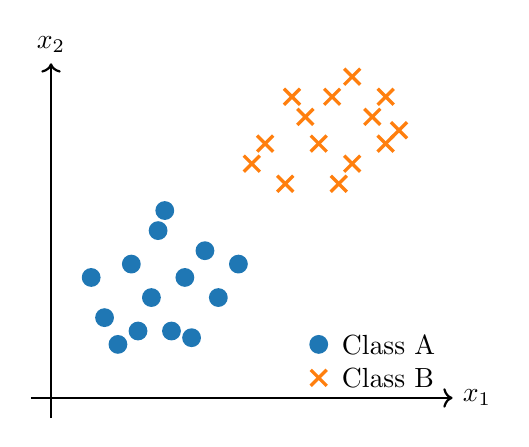
\begin{tikzpicture}[scale=0.85]
                % Axes
                \draw[->, thick] (-0.3,0) -- (6,0) node[right] {$x_1$};
                \draw[->, thick] (0,-0.3) -- (0,5) node[above] {$x_2$};

                % Class A points (blue dots) - clustered lower-left
                \foreach \x/\y in {0.8/1.2, 1.0/0.8, 1.5/1.5, 1.2/2.0, 1.8/1.0,
                                   2.0/1.8, 1.6/2.5, 2.3/2.2, 0.6/1.8, 2.5/1.5,
                                   1.3/1.0, 2.1/0.9, 1.7/2.8, 2.8/2.0} {
                    \fill[classA] (\x,\y) circle (4pt);
                }

                % Class B points (orange crosses) - clustered upper-right
                \foreach \x/\y in {3.5/3.2, 4.0/3.8, 4.5/3.5, 3.8/4.2, 4.2/4.5,
                                   5.0/3.8, 4.8/4.2, 3.2/3.8, 4.5/4.8, 5.2/4.0,
                                   3.6/4.5, 5.0/4.5, 4.3/3.2, 3.0/3.5} {
                    \draw[classB, very thick] (\x-0.12,\y-0.12) -- (\x+0.12,\y+0.12);
                    \draw[classB, very thick] (\x-0.12,\y+0.12) -- (\x+0.12,\y-0.12);
                }

                % Legend
                \fill[classA] (4.0,0.8) circle (4pt);
                \node[right] at (4.2,0.8) {Class A};
                \draw[classB, very thick] (4.0-0.12,0.3-0.12) -- (4.0+0.12,0.3+0.12);
                \draw[classB, very thick] (4.0-0.12,0.3+0.12) -- (4.0+0.12,0.3-0.12);
                \node[right] at (4.2,0.3) {Class B};
            \end{tikzpicture}
        \end{column}
        \begin{column}{0.42\textwidth}
            \textbf{Goal:} Learn a function $f: \mathbb{R}^d \to \{A, B\}$

            \vspace{1em}
            Given training data with features and labels, find decision boundaries that separate the classes.

            \vspace{1em}
            \textbf{Key question:} How do we decide where to split?
        \end{column}
    \end{columns}
\end{frame}

% -----------------------------------------------------------------------------
% Slide 3: Gini Impurity Formula + Curve (from random-forest.tex)
% -----------------------------------------------------------------------------
\begin{frame}{Gini Impurity: Measuring ``Mixedness''}
    \begin{columns}
        \begin{column}{0.48\textwidth}
            \textbf{Definition:}
            \[
            \text{Gini}(S) = 1 - \sum_{i=1}^{k} p_i^2
            \]

            \vspace{0.5em}
            \textbf{For binary classification} ($p$ = proportion of class A):
            \[
            \text{Gini}(S) = 1 - p^2 - (1-p)^2
            \]

            \vspace{1em}
            \begin{itemize}
                \item $\text{Gini} = 0$: Pure node (all one class)
                \item $\text{Gini} = 0.5$: Maximum impurity (50-50 split)
            \end{itemize}
        \end{column}
        \begin{column}{0.48\textwidth}
            \centering
            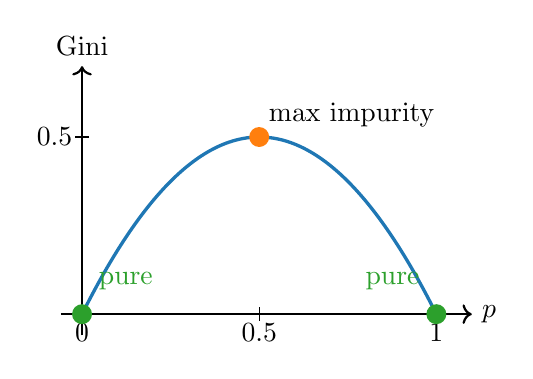
\begin{tikzpicture}[scale=0.9]
                % Axes
                \draw[->, thick] (-0.3,0) -- (5.5,0) node[right] {$p$};
                \draw[->, thick] (0,-0.3) -- (0,3.5) node[above] {Gini};

                % Axis labels
                \node[below] at (0,0) {0};
                \node[below] at (2.5,0) {0.5};
                \node[below] at (5,0) {1};
                \node[left] at (0,2.5) {0.5};

                % Tick marks
                \draw (2.5,0.1) -- (2.5,-0.1);
                \draw (5,0.1) -- (5,-0.1);
                \draw (0.1,2.5) -- (-0.1,2.5);

                % Gini curve: 2p(1-p) scaled
                \draw[classA, very thick, domain=0:5, samples=100]
                    plot (\x, {2*(\x/5)*(1-\x/5)*5});

                % Maximum point
                \fill[classB] (2.5,2.5) circle (4pt);
                \node[above right] at (2.5,2.5) {max impurity};

                % Pure nodes
                \fill[splitline] (0,0) circle (4pt);
                \fill[splitline] (5,0) circle (4pt);
                \node[above right, splitline] at (0.1,0.2) {pure};
                \node[above left, splitline] at (4.9,0.2) {pure};
            \end{tikzpicture}

            \vspace{0.5em}
            \small Gini impurity is maximized when classes are equally mixed
        \end{column}
    \end{columns}
\end{frame}

% -----------------------------------------------------------------------------
% Slide 4: Dataset (from gini_impurity.tex)
% -----------------------------------------------------------------------------
\begin{frame}{Worked Example: Dataset}

\centering
\begin{tabular}{cccc}
\toprule
Sample & Feature A & Feature B & Label \\
\midrule
1 & 0 & 1 & 0 \\
2 & 0 & 0 & 0 \\
3 & 0 & 1 & 0 \\
4 & 1 & 0 & 0 \\
5 & 1 & 1 & 1 \\
6 & 1 & 0 & 1 \\
7 & 1 & 1 & 1 \\
8 & 1 & 1 & 1 \\
\bottomrule
\end{tabular}

\vspace{1em}

\textbf{Label distribution:} 4 samples with Label=0, 4 samples with Label=1

\vspace{0.5em}

\textbf{Goal:} Find the best feature to split on at the root node

\end{frame}

% -----------------------------------------------------------------------------
% Slide 5: Parent Node Gini (from gini_impurity.tex)
% -----------------------------------------------------------------------------
\begin{frame}{Parent Node Gini Impurity}

\textbf{Class proportions:}
\[
p_0 = \frac{4}{8} = 0.5, \quad p_1 = \frac{4}{8} = 0.5
\]

\pause
\vspace{1em}

\textbf{Gini calculation:}
\[
\text{Gini}(\text{parent}) = 1 - 0.5^2 - 0.5^2 = 1 - 0.25 - 0.25 = 0.5
\]

\pause
\vspace{1em}

\textbf{Interpretation:} Maximum impurity (50/50 split between classes)

\end{frame}

% -----------------------------------------------------------------------------
% Slide 6: Split on Feature A (from gini_impurity.tex)
% -----------------------------------------------------------------------------
\begin{frame}{Split on Feature A}

\textbf{Left child (Feature A = 0):} Samples 1, 2, 3 $\rightarrow$ Labels: 0, 0, 0
\[
\text{Gini}(\text{left}) = 1 - 1^2 - 0^2 = 0 \quad \text{(pure node)}
\]

\pause
\vspace{0.5em}

\textbf{Right child (Feature A = 1):} Samples 4, 5, 6, 7, 8 $\rightarrow$ Labels: 0, 1, 1, 1, 1
\[
p_0 = 0.2, \quad p_1 = 0.8
\]
\[
\text{Gini}(\text{right}) = 1 - 0.2^2 - 0.8^2 = 0.32
\]

\pause
\vspace{0.5em}

\textbf{Weighted Gini:}
\[
\text{Gini}_A = \frac{3}{8} \times 0 + \frac{5}{8} \times 0.32 = 0.2
\]

\end{frame}

% -----------------------------------------------------------------------------
% Slide 7: Split on Feature B (from gini_impurity.tex)
% -----------------------------------------------------------------------------
\begin{frame}{Split on Feature B}

\textbf{Left child (Feature B = 0):} Samples 2, 4, 6 $\rightarrow$ Labels: 0, 0, 1
\[
\text{Gini}(\text{left}) = 1 - \left(\frac{2}{3}\right)^2 - \left(\frac{1}{3}\right)^2 = \frac{4}{9} \approx 0.444
\]

\pause
\vspace{0.5em}

\textbf{Right child (Feature B = 1):} Samples 1, 3, 5, 7, 8 $\rightarrow$ Labels: 0, 0, 1, 1, 1
\[
\text{Gini}(\text{right}) = 1 - 0.4^2 - 0.6^2 = 0.48
\]

\pause
\vspace{0.5em}

\textbf{Weighted Gini:}
\[
\text{Gini}_B = \frac{3}{8} \times 0.444 + \frac{5}{8} \times 0.48 = 0.467
\]

\end{frame}

% -----------------------------------------------------------------------------
% Slide 8: Comparison & Decision (from gini_impurity.tex)
% -----------------------------------------------------------------------------
\begin{frame}{Comparison \& Decision}

\centering
\begin{tabular}{lc}
\toprule
Split & Weighted Gini \\
\midrule
Feature A & \textbf{0.200} \\
Feature B & 0.467 \\
\bottomrule
\end{tabular}

\vspace{1.5em}

\pause

\textbf{Decision:} Split on Feature A (lower Gini impurity)

\vspace{1em}

Feature A perfectly separates all Label=0 samples, while Feature B mixes classes in both children.

\end{frame}

% -----------------------------------------------------------------------------
% Slide 9: Building the Tree (from random-forest.tex)
% -----------------------------------------------------------------------------
\begin{frame}{Building the Tree}
    \begin{columns}
        \begin{column}{0.45\textwidth}
            \centering
            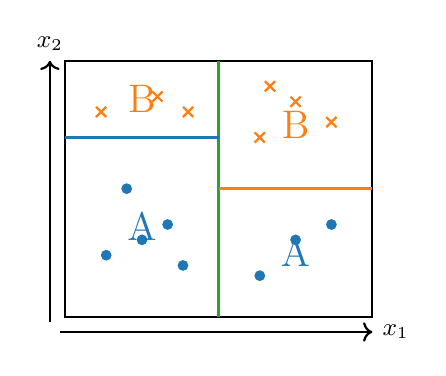
\begin{tikzpicture}[scale=0.65]
                % Feature space with splits
                \draw[thick] (0,0) rectangle (6,5);
                \draw[->, thick] (-0.1,-0.3) -- (6,-0.3) node[right] {\small $x_1$};
                \draw[->, thick] (-0.3,-0.1) -- (-0.3,5) node[above] {\small $x_2$};

                % First split (vertical)
                \draw[splitline, very thick] (3,0) -- (3,5);

                % Second split (horizontal, right side)
                \draw[classB, very thick] (3,2.5) -- (6,2.5);

                % Third split (horizontal, left side)
                \draw[classA, very thick] (0,3.5) -- (3,3.5);

                % Region labels
                \node at (1.5,1.75) {\Large\textcolor{classA}{A}};
                \node at (1.5,4.25) {\Large\textcolor{classB}{B}};
                \node at (4.5,1.25) {\Large\textcolor{classA}{A}};
                \node at (4.5,3.75) {\Large\textcolor{classB}{B}};

                % Data points (sparse for clarity)
                \foreach \x/\y in {0.8/1.2, 1.5/1.5, 2.0/1.8, 1.2/2.5, 2.3/1.0} {
                    \fill[classA] (\x,\y) circle (3pt);
                }
                \foreach \x/\y in {0.7/4.0, 1.8/4.3, 2.4/4.0} {
                    \draw[classB, thick] (\x-0.1,\y-0.1) -- (\x+0.1,\y+0.1);
                    \draw[classB, thick] (\x-0.1,\y+0.1) -- (\x+0.1,\y-0.1);
                }
                \foreach \x/\y in {3.8/0.8, 4.5/1.5, 5.2/1.8} {
                    \fill[classA] (\x,\y) circle (3pt);
                }
                \foreach \x/\y in {3.8/3.5, 4.5/4.2, 5.2/3.8, 4.0/4.5} {
                    \draw[classB, thick] (\x-0.1,\y-0.1) -- (\x+0.1,\y+0.1);
                    \draw[classB, thick] (\x-0.1,\y+0.1) -- (\x+0.1,\y-0.1);
                }
            \end{tikzpicture}

            \small Feature space partitioning
        \end{column}
        \begin{column}{0.52\textwidth}
            \centering
            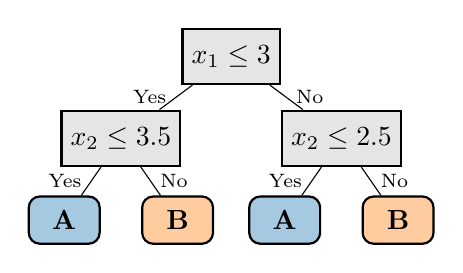
\begin{tikzpicture}[
                scale=0.8,
                level 1/.style={sibling distance=3.5cm, level distance=1.3cm},
                level 2/.style={sibling distance=1.8cm, level distance=1.3cm},
                every node/.style={align=center},
                decision/.style={rectangle, draw, thick, minimum width=1.2cm, minimum height=0.7cm},
                leaf/.style={rectangle, rounded corners, draw, thick, minimum width=0.9cm, minimum height=0.6cm}
            ]
                \node[decision, fill=gray!20] {$x_1 \leq 3$}
                    child {
                        node[decision, fill=gray!20] {$x_2 \leq 3.5$}
                        child {
                            node[leaf, fill=classA!40] {\textbf{A}}
                            edge from parent node[left, font=\scriptsize] {Yes}
                        }
                        child {
                            node[leaf, fill=classB!40] {\textbf{B}}
                            edge from parent node[right, font=\scriptsize] {No}
                        }
                        edge from parent node[left, font=\scriptsize] {Yes}
                    }
                    child {
                        node[decision, fill=gray!20] {$x_2 \leq 2.5$}
                        child {
                            node[leaf, fill=classA!40] {\textbf{A}}
                            edge from parent node[left, font=\scriptsize] {Yes}
                        }
                        child {
                            node[leaf, fill=classB!40] {\textbf{B}}
                            edge from parent node[right, font=\scriptsize] {No}
                        }
                        edge from parent node[right, font=\scriptsize] {No}
                    };
            \end{tikzpicture}

            \vspace{0.5em}
            \small Corresponding decision tree

            \vspace{0.5em}
            Each split uses Gini to find the best feature and threshold
        \end{column}
    \end{columns}
\end{frame}

% -----------------------------------------------------------------------------
% Slide 10: Bootstrap Sampling (from random-forest.tex)
% -----------------------------------------------------------------------------
\begin{frame}{Bootstrap Sampling: Creating Diverse Training Sets}
    \centering
    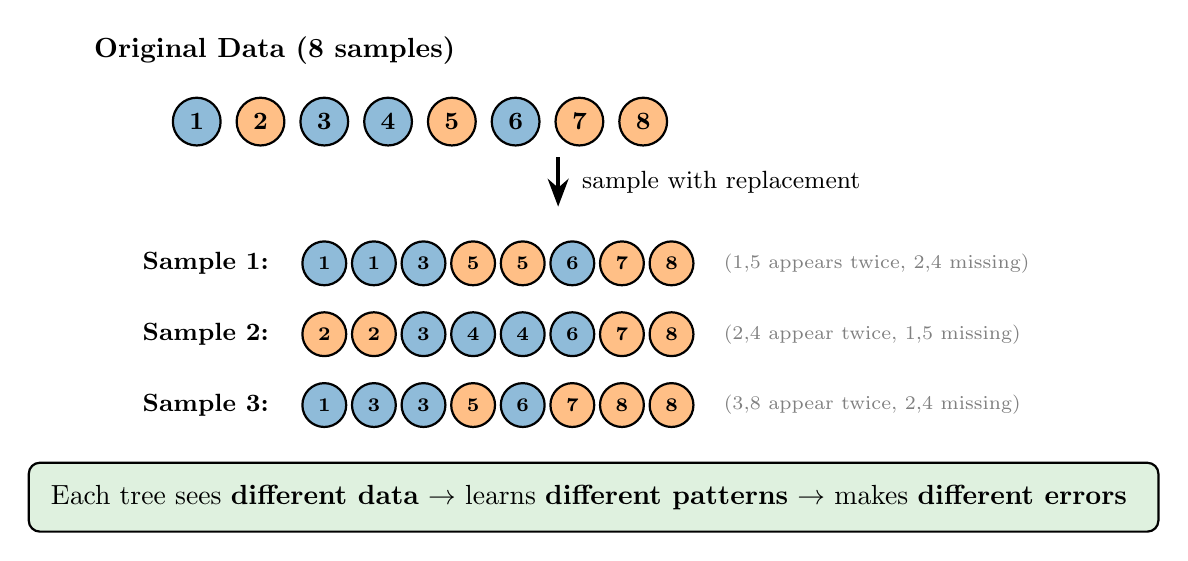
\begin{tikzpicture}[scale=0.9]
        % Original dataset
        \node[font=\bfseries] at (-4.5,3) {Original Data (8 samples)};
        \foreach \i/\col in {1/classA, 2/classB, 3/classA, 4/classA, 5/classB, 6/classA, 7/classB, 8/classB} {
            \node[circle, draw, thick, fill=\col!50, minimum size=0.6cm, font=\small\bfseries]
                (orig\i) at (-6.5+\i*0.9, 2) {\i};
        }

        % Arrow to bootstrap samples
        \draw[-{Stealth[scale=1.2]}, very thick] (-0.5,1.5) -- (-0.5,0.8);
        \node[right, font=\small] at (-0.3,1.15) {sample with replacement};

        % Bootstrap sample 1
        \node[font=\small\bfseries, anchor=west] at (-6.5,0) {Sample 1:};
        \foreach \i/\val/\col in {1/1/classA, 2/1/classA, 3/3/classA, 4/5/classB, 5/5/classB, 6/6/classA, 7/7/classB, 8/8/classB} {
            \node[circle, draw, thick, fill=\col!50, minimum size=0.5cm, font=\scriptsize\bfseries]
                at (-4.5+\i*0.7, 0) {\val};
        }
        \node[font=\scriptsize, gray, anchor=west] at (1.7,0) {(1,5 appears twice, 2,4 missing)};

        % Bootstrap sample 2
        \node[font=\small\bfseries, anchor=west] at (-6.5,-1) {Sample 2:};
        \foreach \i/\val/\col in {1/2/classB, 2/2/classB, 3/3/classA, 4/4/classA, 5/4/classA, 6/6/classA, 7/7/classB, 8/8/classB} {
            \node[circle, draw, thick, fill=\col!50, minimum size=0.5cm, font=\scriptsize\bfseries]
                at (-4.5+\i*0.7, -1) {\val};
        }
        \node[font=\scriptsize, gray, anchor=west] at (1.7,-1) {(2,4 appear twice, 1,5 missing)};

        % Bootstrap sample 3
        \node[font=\small\bfseries, anchor=west] at (-6.5,-2) {Sample 3:};
        \foreach \i/\val/\col in {1/1/classA, 2/3/classA, 3/3/classA, 4/5/classB, 5/6/classA, 6/7/classB, 7/8/classB, 8/8/classB} {
            \node[circle, draw, thick, fill=\col!50, minimum size=0.5cm, font=\scriptsize\bfseries]
                at (-4.5+\i*0.7, -2) {\val};
        }
        \node[font=\scriptsize, gray, anchor=west] at (1.7,-2) {(3,8 appear twice, 2,4 missing)};

        % Key insight box
        \node[draw, thick, rounded corners, fill=splitline!15, inner sep=8pt, align=left] at (0,-3.3) {
            Each tree sees \textbf{different data} $\rightarrow$ learns \textbf{different patterns} $\rightarrow$ makes \textbf{different errors}
        };
    \end{tikzpicture}
\end{frame}

% -----------------------------------------------------------------------------
% Slide 11: Different Data → Different Trees (from random-forest.tex)
% -----------------------------------------------------------------------------
\begin{frame}{Different Data $\rightarrow$ Different Trees}
    \centering
    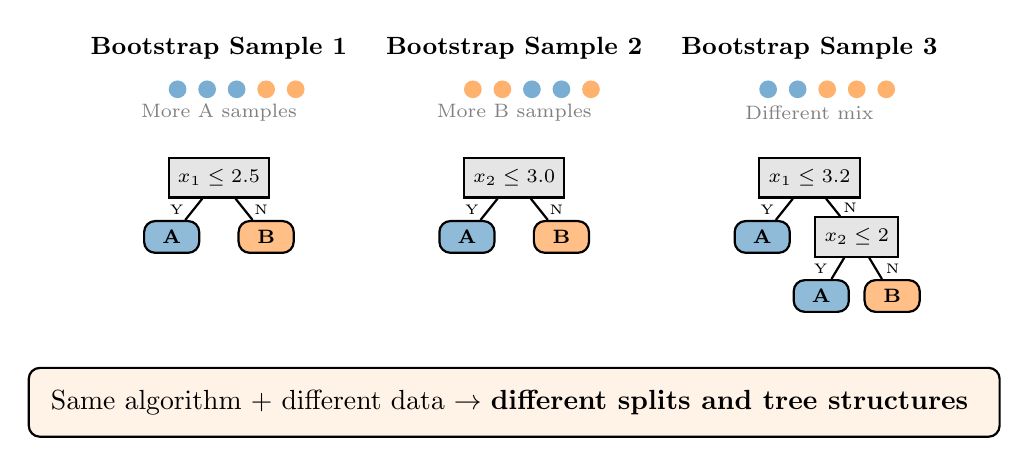
\begin{tikzpicture}[
        scale=0.75,
        decision/.style={rectangle, draw, thick, fill=gray!20, minimum width=1cm, minimum height=0.5cm, font=\scriptsize},
        leaf/.style={rectangle, rounded corners, draw, thick, minimum width=0.7cm, minimum height=0.4cm, font=\scriptsize\bfseries}
    ]
        % Sample 1 and its tree
        \begin{scope}[shift={(-5,0)}]
            \node[font=\small\bfseries] at (0,3.2) {Bootstrap Sample 1};
            % Mini data representation
            \foreach \i/\col in {1/classA, 2/classA, 3/classA, 4/classB, 5/classB} {
                \fill[\col!60] (-1.2+\i*0.5, 2.5) circle (0.15);
            }
            \node[font=\scriptsize, gray] at (0,2.1) {More A samples};

            % Tree 1: splits at x1 ≤ 2.5
            \node[decision] (t1root) at (0,1) {$x_1 \leq 2.5$};
            \node[leaf, fill=classA!50] (t1l) at (-0.8,0) {A};
            \node[leaf, fill=classB!50] (t1r) at (0.8,0) {B};
            \draw[thick] (t1root) -- (t1l) node[midway, left, font=\tiny] {Y};
            \draw[thick] (t1root) -- (t1r) node[midway, right, font=\tiny] {N};
        \end{scope}

        % Sample 2 and its tree
        \begin{scope}[shift={(0,0)}]
            \node[font=\small\bfseries] at (0,3.2) {Bootstrap Sample 2};
            % Mini data representation
            \foreach \i/\col in {1/classB, 2/classB, 3/classA, 4/classA, 5/classB} {
                \fill[\col!60] (-1.2+\i*0.5, 2.5) circle (0.15);
            }
            \node[font=\scriptsize, gray] at (0,2.1) {More B samples};

            % Tree 2: splits at x2 ≤ 3.0
            \node[decision] (t2root) at (0,1) {$x_2 \leq 3.0$};
            \node[leaf, fill=classA!50] (t2l) at (-0.8,0) {A};
            \node[leaf, fill=classB!50] (t2r) at (0.8,0) {B};
            \draw[thick] (t2root) -- (t2l) node[midway, left, font=\tiny] {Y};
            \draw[thick] (t2root) -- (t2r) node[midway, right, font=\tiny] {N};
        \end{scope}

        % Sample 3 and its tree
        \begin{scope}[shift={(5,0)}]
            \node[font=\small\bfseries] at (0,3.2) {Bootstrap Sample 3};
            % Mini data representation
            \foreach \i/\col in {1/classA, 2/classA, 3/classB, 4/classB, 5/classB} {
                \fill[\col!60] (-1.2+\i*0.5, 2.5) circle (0.15);
            }
            \node[font=\scriptsize, gray] at (0,2.1) {Different mix};

            % Tree 3: splits at x1 ≤ 3.2
            \node[decision] (t3root) at (0,1) {$x_1 \leq 3.2$};
            \node[leaf, fill=classA!50] (t3l) at (-0.8,0) {A};
            \node[decision] (t3r) at (0.8,0) {$x_2 \leq 2$};
            \node[leaf, fill=classA!50] (t3rl) at (0.2,-1) {A};
            \node[leaf, fill=classB!50] (t3rr) at (1.4,-1) {B};
            \draw[thick] (t3root) -- (t3l) node[midway, left, font=\tiny] {Y};
            \draw[thick] (t3root) -- (t3r) node[midway, right, font=\tiny] {N};
            \draw[thick] (t3r) -- (t3rl) node[midway, left, font=\tiny] {Y};
            \draw[thick] (t3r) -- (t3rr) node[midway, right, font=\tiny] {N};
        \end{scope}

        % Bottom annotation
        \node[draw, thick, rounded corners, fill=classB!10, inner sep=8pt, align=center] at (0,-2.8) {
            Same algorithm + different data $\rightarrow$ \textbf{different splits and tree structures}
        };
    \end{tikzpicture}
\end{frame}

% -----------------------------------------------------------------------------
% Slide 12: Aggregation - Majority Voting (from random-forest.tex)
% -----------------------------------------------------------------------------
\begin{frame}{Aggregation: Majority Voting}
    \centering
    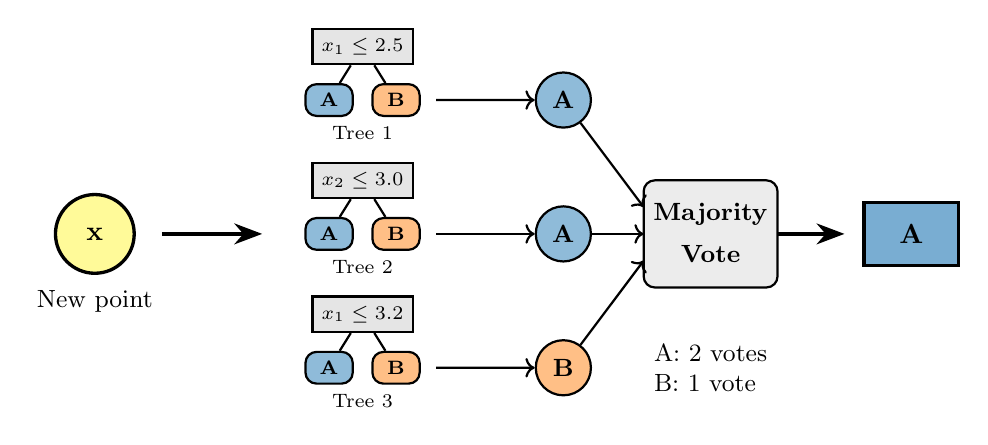
\begin{tikzpicture}[
        scale=0.85,
        decision/.style={rectangle, draw, thick, fill=gray!20, minimum width=0.9cm, minimum height=0.45cm, font=\scriptsize},
        leaf/.style={rectangle, rounded corners, draw, thick, minimum width=0.6cm, minimum height=0.35cm, font=\scriptsize\bfseries}
    ]
        % Input
        \node[circle, draw, very thick, fill=yellow!40, minimum size=1cm] (input) at (-5,0) {$\mathbf{x}$};
        \node[below, font=\small] at (-5,-0.7) {New point};

        % Arrow to trees
        \draw[-{Stealth[scale=1.2]}, very thick] (-4,0) -- (-2.5,0);

        % Tree 1
        \begin{scope}[shift={(-1,2)}]
            \node[decision] (r1) at (0,0.8) {$x_1 \leq 2.5$};
            \node[leaf, fill=classA!50] (l1a) at (-0.5,0) {A};
            \node[leaf, fill=classB!50] (l1b) at (0.5,0) {B};
            \draw[thick] (r1) -- (l1a);
            \draw[thick] (r1) -- (l1b);
            \node[font=\scriptsize, below] at (0,-0.25) {Tree 1};
        \end{scope}

        % Tree 2
        \begin{scope}[shift={(-1,0)}]
            \node[decision] (r2) at (0,0.8) {$x_2 \leq 3.0$};
            \node[leaf, fill=classA!50] (l2a) at (-0.5,0) {A};
            \node[leaf, fill=classB!50] (l2b) at (0.5,0) {B};
            \draw[thick] (r2) -- (l2a);
            \draw[thick] (r2) -- (l2b);
            \node[font=\scriptsize, below] at (0,-0.25) {Tree 2};
        \end{scope}

        % Tree 3
        \begin{scope}[shift={(-1,-2)}]
            \node[decision] (r3) at (0,0.8) {$x_1 \leq 3.2$};
            \node[leaf, fill=classA!50] (l3a) at (-0.5,0) {A};
            \node[leaf, fill=classB!50] (l3b) at (0.5,0) {B};
            \draw[thick] (r3) -- (l3a);
            \draw[thick] (r3) -- (l3b);
            \node[font=\scriptsize, below] at (0,-0.25) {Tree 3};
        \end{scope}

        % Votes
        \node[circle, draw, thick, fill=classA!50, minimum size=0.7cm, font=\small\bfseries] (v1) at (2,2) {A};
        \node[circle, draw, thick, fill=classA!50, minimum size=0.7cm, font=\small\bfseries] (v2) at (2,0) {A};
        \node[circle, draw, thick, fill=classB!50, minimum size=0.7cm, font=\small\bfseries] (v3) at (2,-2) {B};

        % Arrows from trees to votes
        \draw[->, thick] (0.1,2) -- (v1);
        \draw[->, thick] (0.1,0) -- (v2);
        \draw[->, thick] (0.1,-2) -- (v3);

        % Aggregation box
        \draw[thick, rounded corners, fill=gray!15] (3.2,-0.8) rectangle (5.2,0.8);
        \node[align=center, font=\small] at (4.2,0.3) {\textbf{Majority}};
        \node[align=center, font=\small] at (4.2,-0.3) {\textbf{Vote}};

        % Arrows to aggregation
        \draw[->, thick] (v1) -- (3.2,0.4);
        \draw[->, thick] (v2) -- (3.2,0);
        \draw[->, thick] (v3) -- (3.2,-0.4);

        % Final output
        \draw[-{Stealth[scale=1.2]}, very thick] (5.2,0) -- (6.2,0);
        \node[rectangle, draw, very thick, fill=classA!60, minimum width=1.2cm, minimum height=0.8cm, font=\bfseries] at (7.2,0) {A};

        % Vote tally
        \node[align=left, font=\small] at (4.2,-2) {
            A: 2 votes\\
            B: 1 vote
        };
    \end{tikzpicture}

    \vspace{1em}
    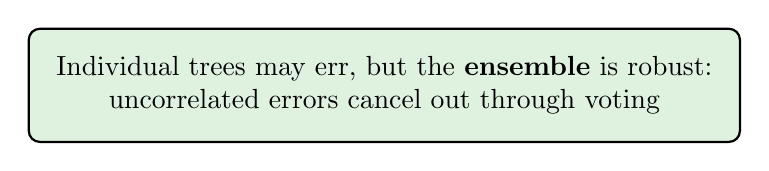
\begin{tikzpicture}
        \node[draw, thick, rounded corners, fill=splitline!15, inner sep=10pt, align=center] {
            Individual trees may err, but the \textbf{ensemble} is robust:\\
            uncorrelated errors cancel out through voting
        };
    \end{tikzpicture}
\end{frame}

% -----------------------------------------------------------------------------
% Slide 13: Summary (combined from both decks)
% -----------------------------------------------------------------------------
\begin{frame}{Summary}
    \centering
    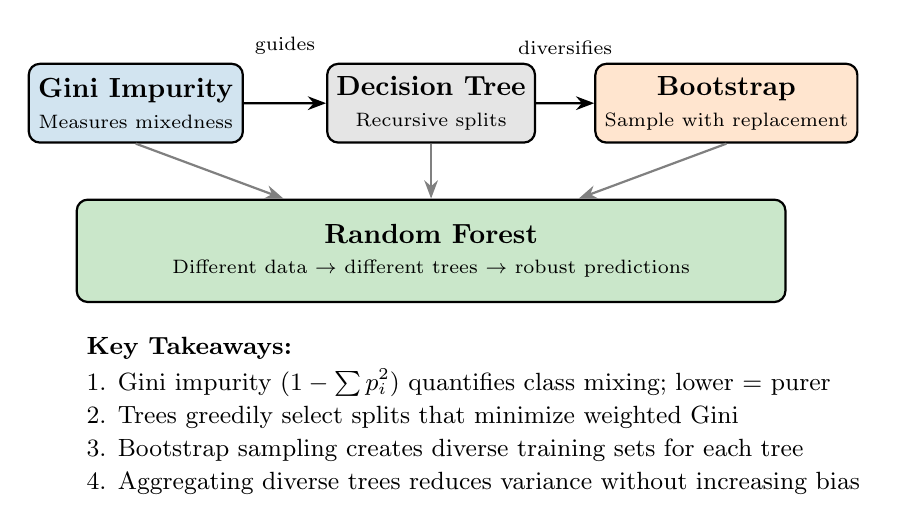
\begin{tikzpicture}[
        scale=0.75,
        box/.style={draw, thick, rounded corners, minimum width=2.5cm, minimum height=1cm, align=center},
        arrow/.style={-{Stealth[scale=1]}, thick}
    ]
        % Row 1: Three concept boxes with more horizontal spacing
        \node[box, fill=classA!20] (gini) at (-5,2) {\textbf{Gini Impurity}\\[-0.1em]\scriptsize Measures mixedness};

        \node[box, fill=gray!20] (tree) at (0,2) {\textbf{Decision Tree}\\[-0.1em]\scriptsize Recursive splits};

        \node[box, fill=classB!20] (boot) at (5,2) {\textbf{Bootstrap}\\[-0.1em]\scriptsize Sample with replacement};

        % Arrows between top row with labels above, offset to clear boxes
        \draw[arrow] (gini) -- (tree) node[midway, above, yshift=14pt, font=\scriptsize] {guides};
        \draw[arrow] (tree) -- (boot) node[midway, above, yshift=14pt, font=\scriptsize] {diversifies};

        % Bottom: Random Forest
        \node[box, fill=splitline!25, minimum width=9cm, minimum height=1.3cm] (forest) at (0,-0.5) {
            \textbf{Random Forest}\\[-0.1em]
            \scriptsize Different data $\rightarrow$ different trees $\rightarrow$ robust predictions
        };

        % Straight arrows down to forest (cleaner than curved)
        \draw[arrow, gray] (gini.south) -- ([xshift=-2.5cm]forest.north);
        \draw[arrow, gray] (tree.south) -- (forest.north);
        \draw[arrow, gray] (boot.south) -- ([xshift=2.5cm]forest.north);

        % Key takeaways
        \node[align=left, anchor=north west, font=\small] at (-6,-1.8) {
            \textbf{Key Takeaways:}\\[0.2em]
            1. Gini impurity ($1 - \sum p_i^2$) quantifies class mixing; lower = purer\\[0.1em]
            2. Trees greedily select splits that minimize weighted Gini\\[0.1em]
            3. Bootstrap sampling creates diverse training sets for each tree\\[0.1em]
            4. Aggregating diverse trees reduces variance without increasing bias
        };
    \end{tikzpicture}

    \vspace{0.3em}
    \colorbox{splitline!20}{\parbox{0.85\textwidth}{\centering
        \textbf{Core principle:} Diversity through bootstrapping transforms high-variance trees into a low-variance ensemble.
    }}
\end{frame}

\end{document}
